\setcounter{chapter}{2}
\setcounter{section}{0}
\setcounter{equation}{0}
\setcounter{figure}{0}
\addcontentsline{toc}{chapter}{Глава 2. Усовершенствованный итеративный алгоритм вычисления оценки АКФ}
\chapter*{Глава 2. Усовершенствованный итеративный алгоритм вычисления оценки АКФ}
\label{l:sec_acf}

\section{Постановка задачи}

Для эффективного использования АР-метода необходимо иметь точную оценку АКФ. Наличие шума в аддитивной смеси ведет к неточной
оценке АКФ, что, в свою очередь, ведет к смещенной оценке резонансных частот. Вычислительная сложность итеративной оценки АКФ является квадратичной
функцией от длинны входной последовательности, поэтому итеративная оценка АКФ для нескольких источников не может быть реализована в программном приемнике
по причине большой ресурсоемкости. В данной главе ставится и решается задача оптимизации алгоритма итеративного вычисления АКФ. Также в данной
главе приводится обоснование возможности и эффективности применения итеративного алгоритма вычисления АКФ для подавления эффектов МКИ и повышения ОСШ сигнала
при оценке частоты в АР-модели. В конце главы представлено численное моделирование.

АКФ, по определению, представляет неслучайную функцию.
Для получения данной функции необходимо обладать бесконечным количеством реализаций или, в случае эргодического процесса, реализацией бесконечной длинны \cite{bolshakov-book}.

Оценка АКФ ${\hat{r}_{xx}(\tau, T)}$ является случайной функцией. Оценка данной функции должна наилучшим образом отражать реальные характеристики процесса.

Из большого числа методов оценки АКФ наиболее часто применяются прямые и косвенные. При использовании прямого метода вычисляется интеграл:
\begin{equation}
	\label{eq:acf_integral_basic}
	\hat{r}_{xx}(\tau, T) = \frac{1}{T-\tau} \int_{0}^{t-\tau} (x(t) - \hat{E}(x))(x(t+\tau) - \hat{E}(x))dt,
\end{equation}
где ${\hat{r}_{xx}(\tau, T)}$ -  оценка автокорреляционной функции. Остальные методы: основанные на интегральном преобразовании Фурье, использующие интеграл вероятностей, принцип
знакосочетаний, компенсации, интерференции, разложения по ортогональным функциям, относятся к косвенным \cite{bolshakov-book}.

Погрешности оценки можно разделить на три группы \cite{bolshakov-book}:
\begin{enumerate}
	\item Методические погрешности. Данные погрешности обусловлены ограниченностью отрезка реализации, шагом дискретизации и шумом квантования;
	\item Инструментальные погрешности. Данный вид погрешностей обусловлен погрешностями: измерительных приборов, записи, хранения, вычислений;
	\item Погрешности от влияния коррелированных и некоррелированных помех.
\end{enumerate}

Подходы к компенсации шума при АР анализе достаточно подробно рассмотрены в классических работах \cite{kay_ar_book, kay_noise_compensation}.
При наличии АБГШ во входной смеси ${x(m)}$ ее АКФ может быть записана как:
\begin{equation}
	\label{eq:acf_noise_basic}
	r_{xx}(m) =	\begin{cases}
				r_{ss}(0) + \sigma_n^2, & \mbox{если } m=0; \\
				r_{ss}(m), & \mbox{если } m \ne 0,
			\end{cases}
\end{equation}
где ${r_{ss}(m)}$ - АКФ гармонического сигнала 
Если вычесть ${\sigma_n^2}$ из ${r_{xx}(0)}$ в (\ref{eq:acf_noise_basic}) параметры АР процесса могут быть найдены. Однако, если ${\sigma_n^2}$ достаточно велика или 
оценка АКФ матрица входной смеси ${{\bf{\hat{R}_{xx}}}}$ плохая, матрица ${{\bf{\hat{R}_{xx}}} - {\bf{I}}\sigma_n^2}$ может быть не положительно определена. В данном
случае необходимо вводить поправочный коэффициент. Но для применения данного метода необходимы априорные знания или оценка ${\sigma_n^2}$,
что в случае оценки параметров ШПС в городских условиях (наличие интерференционной помехи от переотражения сигнала, а так же других источников сигнала,
наличие наличие преград на пути распространения сигнала и т.п.) является крайне затруднительным.

Различные методы оценки параметров для АР-модели, основанные на принципе максимального правдоподобия, не
могут считаться ММП при наличии шума в данных. В виду сложности использования ММП, в \cite{marpl_book, kay_ar_book} предложено несколько 
субоптимальных оценок:
\begin{enumerate}
	\item Применение АРСС;
	\item Фильтрация данных для уменьшения мощности шума;
	\item Компенсация параметров АР или оценки коэффициентов отражения;
	\item Использования АР-модели более высокого порядка.
\end{enumerate}

Разрешающая способность оценки частоты при применении АР-модели снижается при снижении уровня ОСШ.
Разрешающую способность оценки АР-модели для гармонических сигналов
одинаковой мощности в случае известной АКФ можно определить приблизительно с помощью формулы Марпла \cite{marpl_book, kay_ar_book}:
\begin{equation}
	\label{eq:lpc_est_quality_1}
	F = \frac{1.03}{Tp[R_e(P+1)]^{0.31}},
\end{equation}
где ${F}$ - разрешение в герцах, ${T}$ - интервал отсчетов в секундах, ${P}$ - порядок модели, ${R_e}$ - ОСШ для отдельного гармонического сигнала, выраженный в линейных единицах.

В работах \cite{lacoss_spectral_est, chen_spectral_est, marple_1977} предложены способы повышения разрешающей способности в задаче оценки спектра входной смеси, но
в данных работах не рассмотрен еще один интересный алгоритм уточнения АКФ - итеративный пересчет АКФ \cite{ostanin_akf}. В данной работе используется
модификация данного алгоритма поэтому целесообразно рассмотреть его подробнее.

В \cite{ostanin_akf} предлагается использовать метод последовательного вычисления АКФ для уточнения оценки АКФ. Данный метод
заключается в последовательном вычислении АКФ от АКФ несколько раз. При этом ОСШ увеличивается от итерации к итерации.
Процесс повторяется несколько раз. Количество итераций зависит от значения ОСШ сигнала. Возможность применения данного подхода в оценке параметров ШПС рассмотрена
автором в \cite{my_acf_cdma}.

%%%%%%%%%%%
\section{Алгоритм итеративного вычисления АКФ}
\label{sec_ostanin}

Пусть входная смесь может быть записана как сумма полезного сигнала ${s(t)}$ и шума ${n(t)}$:
\begin{equation}
	\label{eq:acf_signal}
	x(t) = A \cos{(\omega t)} + n(t)
\end{equation}

Пусть функции ${s(t)}$ и ${n(t)}$ - центрированы. Тогда АКФ выражения (\ref{eq:acf_signal}) может быть записана как \cite{book_max}:
\begin{eqnarray}
	\label{eq:acf_rss_signal}
	r_{xx}(\tau)	& = & \lim_{T \to \infty} \frac{1}{T} \int \limits_0^T x(t)x(t-\tau)dt = \nonumber \\
			& = & \lim_{T \to \infty} \frac{1}{T} \int \limits_0^T (A \cos{(\omega t)} + n(t))(A \cos{(\omega t - \tau)}) + \\
			&   & + n(t - \tau))dt \nonumber
\end{eqnarray}

Тогда, оценка АКФ может быть записана как:
\begin{equation}
	\label{eq:acf_rss_signal_full}
	\hat{r}_{xx}(\tau)=\hat{r}_{ss}(\tau)+\hat{r}_{sn}(\tau)+\hat{r}_{ns}(\tau) + \hat{r}_{nn}(\tau).
\end{equation}

Корреляционные функции ${\hat{r}_{sn}}$ и ${\hat{r}_{ns}}$ тождественно равны 0, с точностью до погрешности, при условии независимости
${x(t)}$ и ${n(t)}$. Таким образом (\ref{eq:acf_signal}) можно переписать:
\begin{equation}
	\label{eq:acf_rss_signal_new}
	\hat{r}_{xx}(t) = \hat{r}_{ss}(t) + \epsilon (t)
\end{equation}

Стоит учесть, что ${\epsilon (t)}$ стремится к нулю с ростом ${T}$. Фурье-образ ${\hat{r}_{xx}(t)}$
представляет собой СПМ, а, следовательно, равен квадрату Фурье-образа исходной функции ${x(t)}$.
Если обозначить ОСШ, выраженное в линейных единицах, сигнала ${x(t)}$ как ${R_s}$, тогда ОСШ после вычисления АКФ может быть выражено 
как \cite{book_max}:
\begin{equation}
	\label{eq:acf_snr_est}
	R_e=2BTR_s \frac{1}{2+1/R_s},
\end{equation}
где ${B}$ - эффективная полоса частот, ${T}$ - длительность, а ${R_s}$ - ОСШ сигнала.

Стоит отметить, что функция ${\epsilon(\tau)}$, как и ${n(t)}$ - является центрированной и
стационарной случайной величиной.
Учитывая, что гармоническая составляющая содержится в ${\hat{r}_{ss}(t)}$, а аддитивный шум в ${\epsilon(\tau)}$, можно провести
следующую итерацию вычисления АКФ. Для оценки ОСШ по формуле (\ref{eq:acf_snr_est}) нужно принять ${R_s' = R_e}$.

Из (\ref{eq:acf_snr_est}) видно, что увеличение ОСШ при вычислении оценки АКФ пропорционально ${2BT}$ и зависит от
ОСШ на входе коррелометра, также можно отметить, что увеличение ОСШ происходит только при условии ${BT > \frac{1}{2R_s} + 1}$.
Оценка прироста ОСШ на ${k}$-ой итерации получается рекуррентно по формуле (\ref{eq:acf_snr_est}).

На Рис. \ref{pic:acf_0_iter} представлен входной сигнал, а на
Рис. \ref{pic:acf_1_iter}, \ref{pic:acf_4_iter} представлены оценки АКФ на первом и четвертом шагах.
Моделирование проводилось для гармонического сигнала при ОСШ -43.82 дБ с нормированной частотой 20 Гц для
отрезка 600 точек.

\begin{figure}[h]
	\center\scalebox{1}{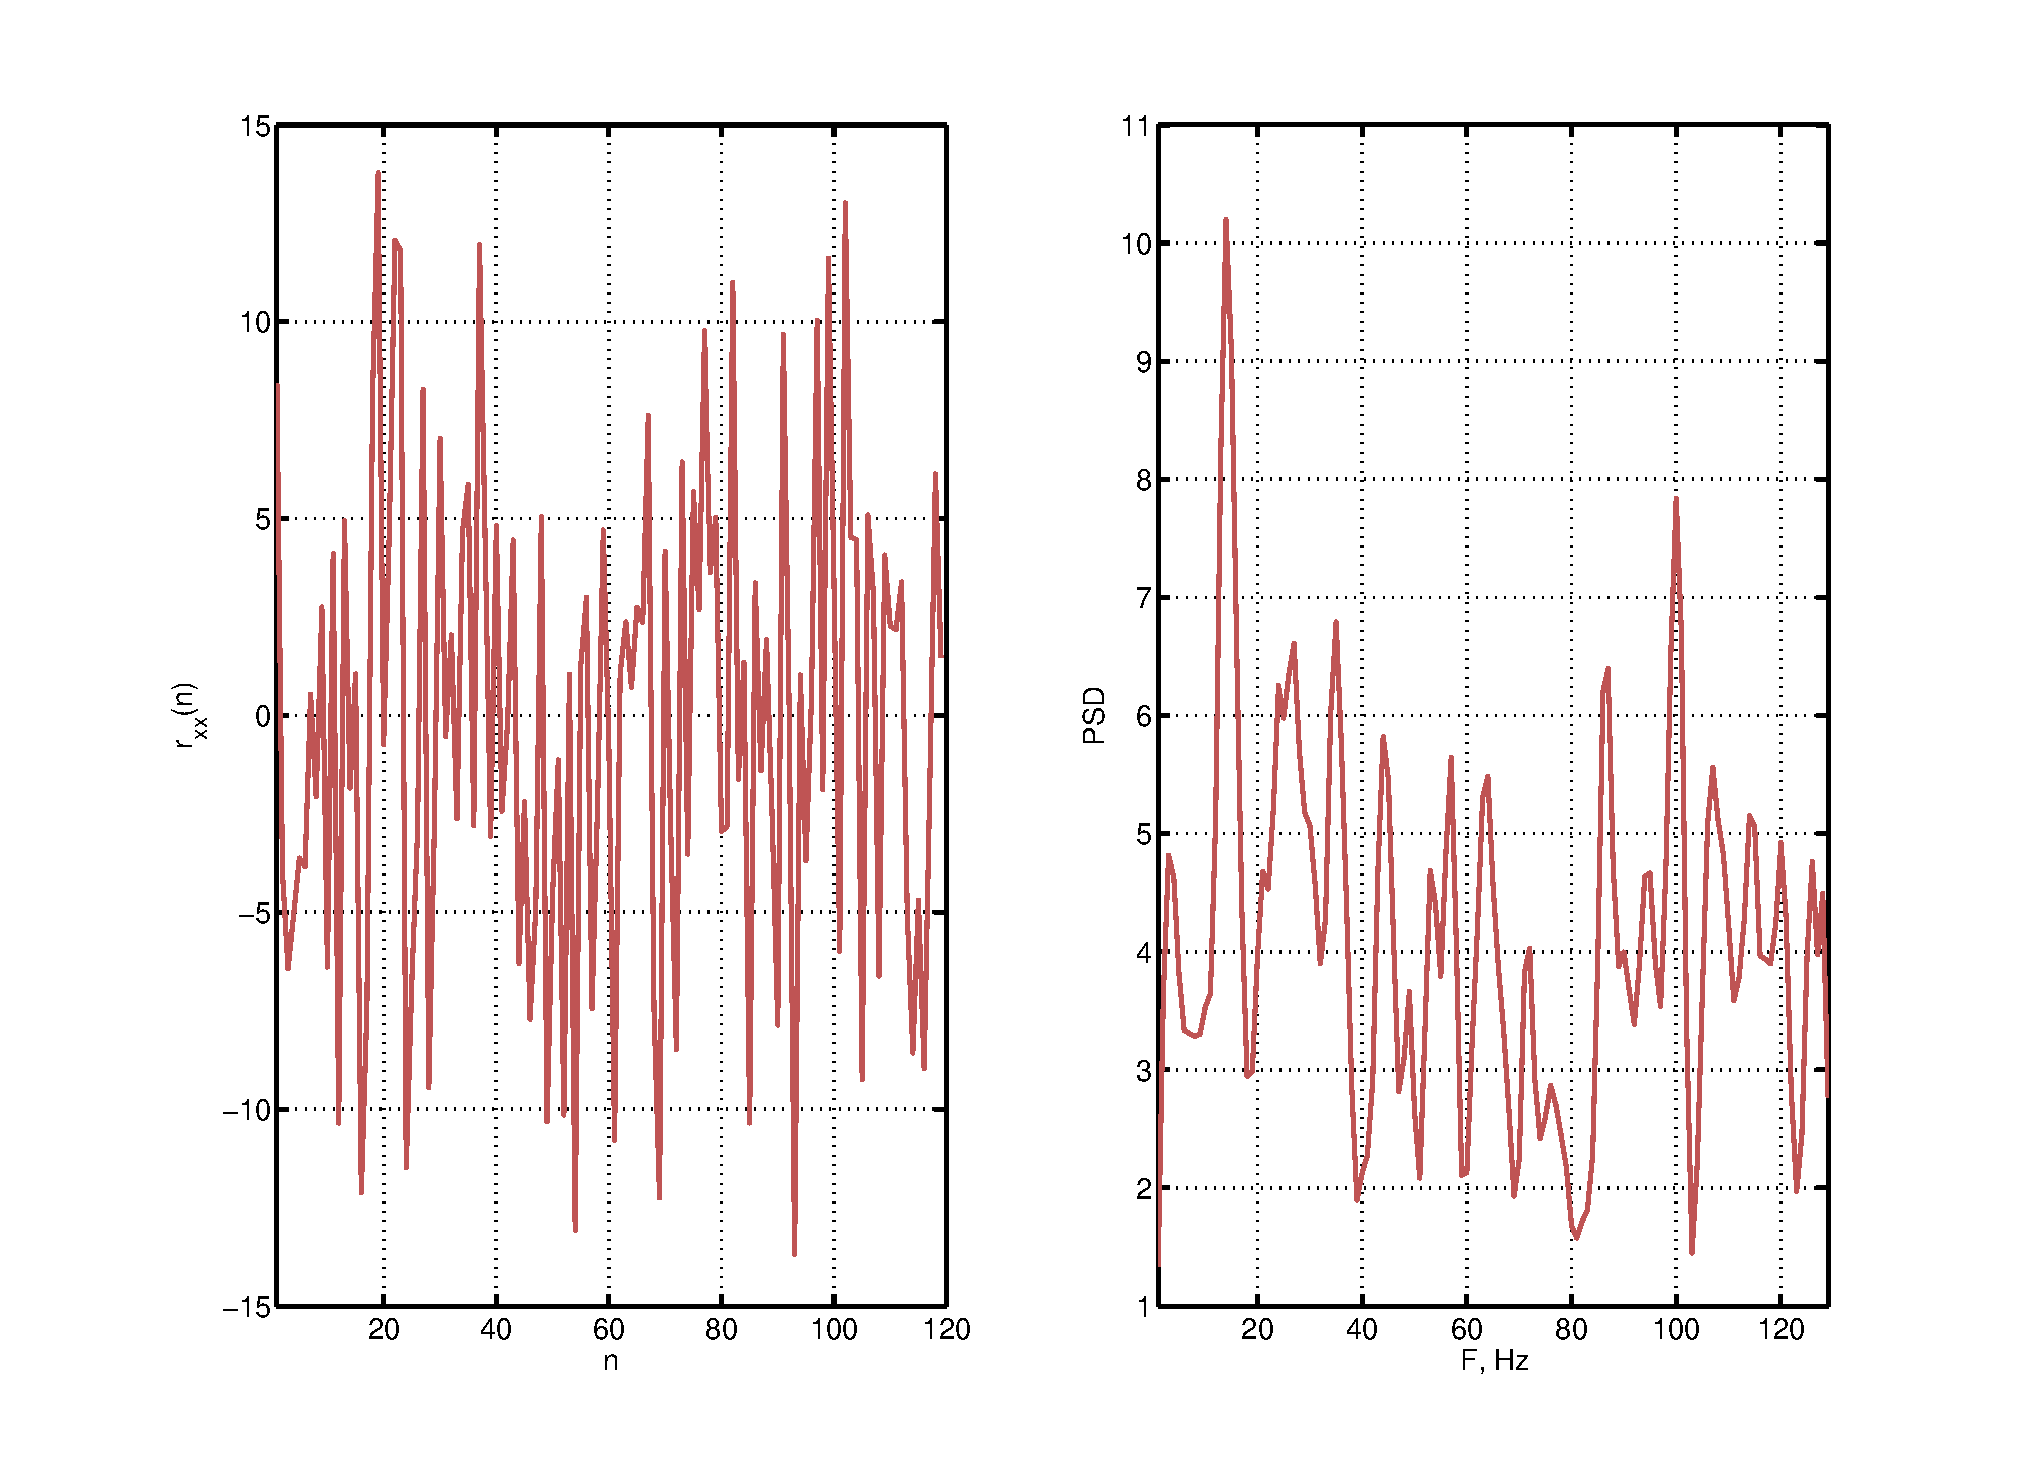
\includegraphics[width=1\linewidth]{acf_0_iter.eps}}
	\caption{Исходный сигнал и его спектр.}
	\label{pic:acf_0_iter}
\end{figure}

\begin{figure}[h]
	\center\scalebox{1}{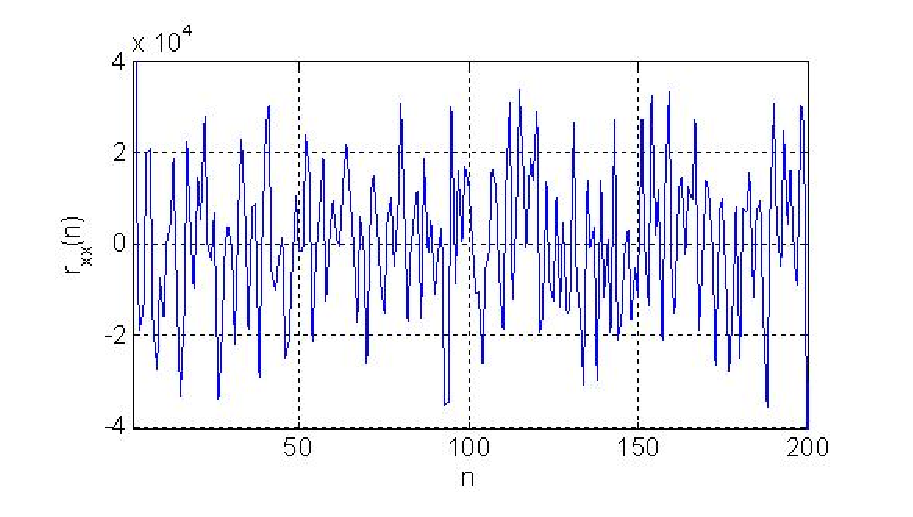
\includegraphics[width=1\linewidth]{acf_1_iter.eps}}
	\caption{Оценка АКФ на 1 итерации и ее спектр.}
	\label{pic:acf_1_iter}
\end{figure}

\begin{figure}[h]
	\center\scalebox{1}{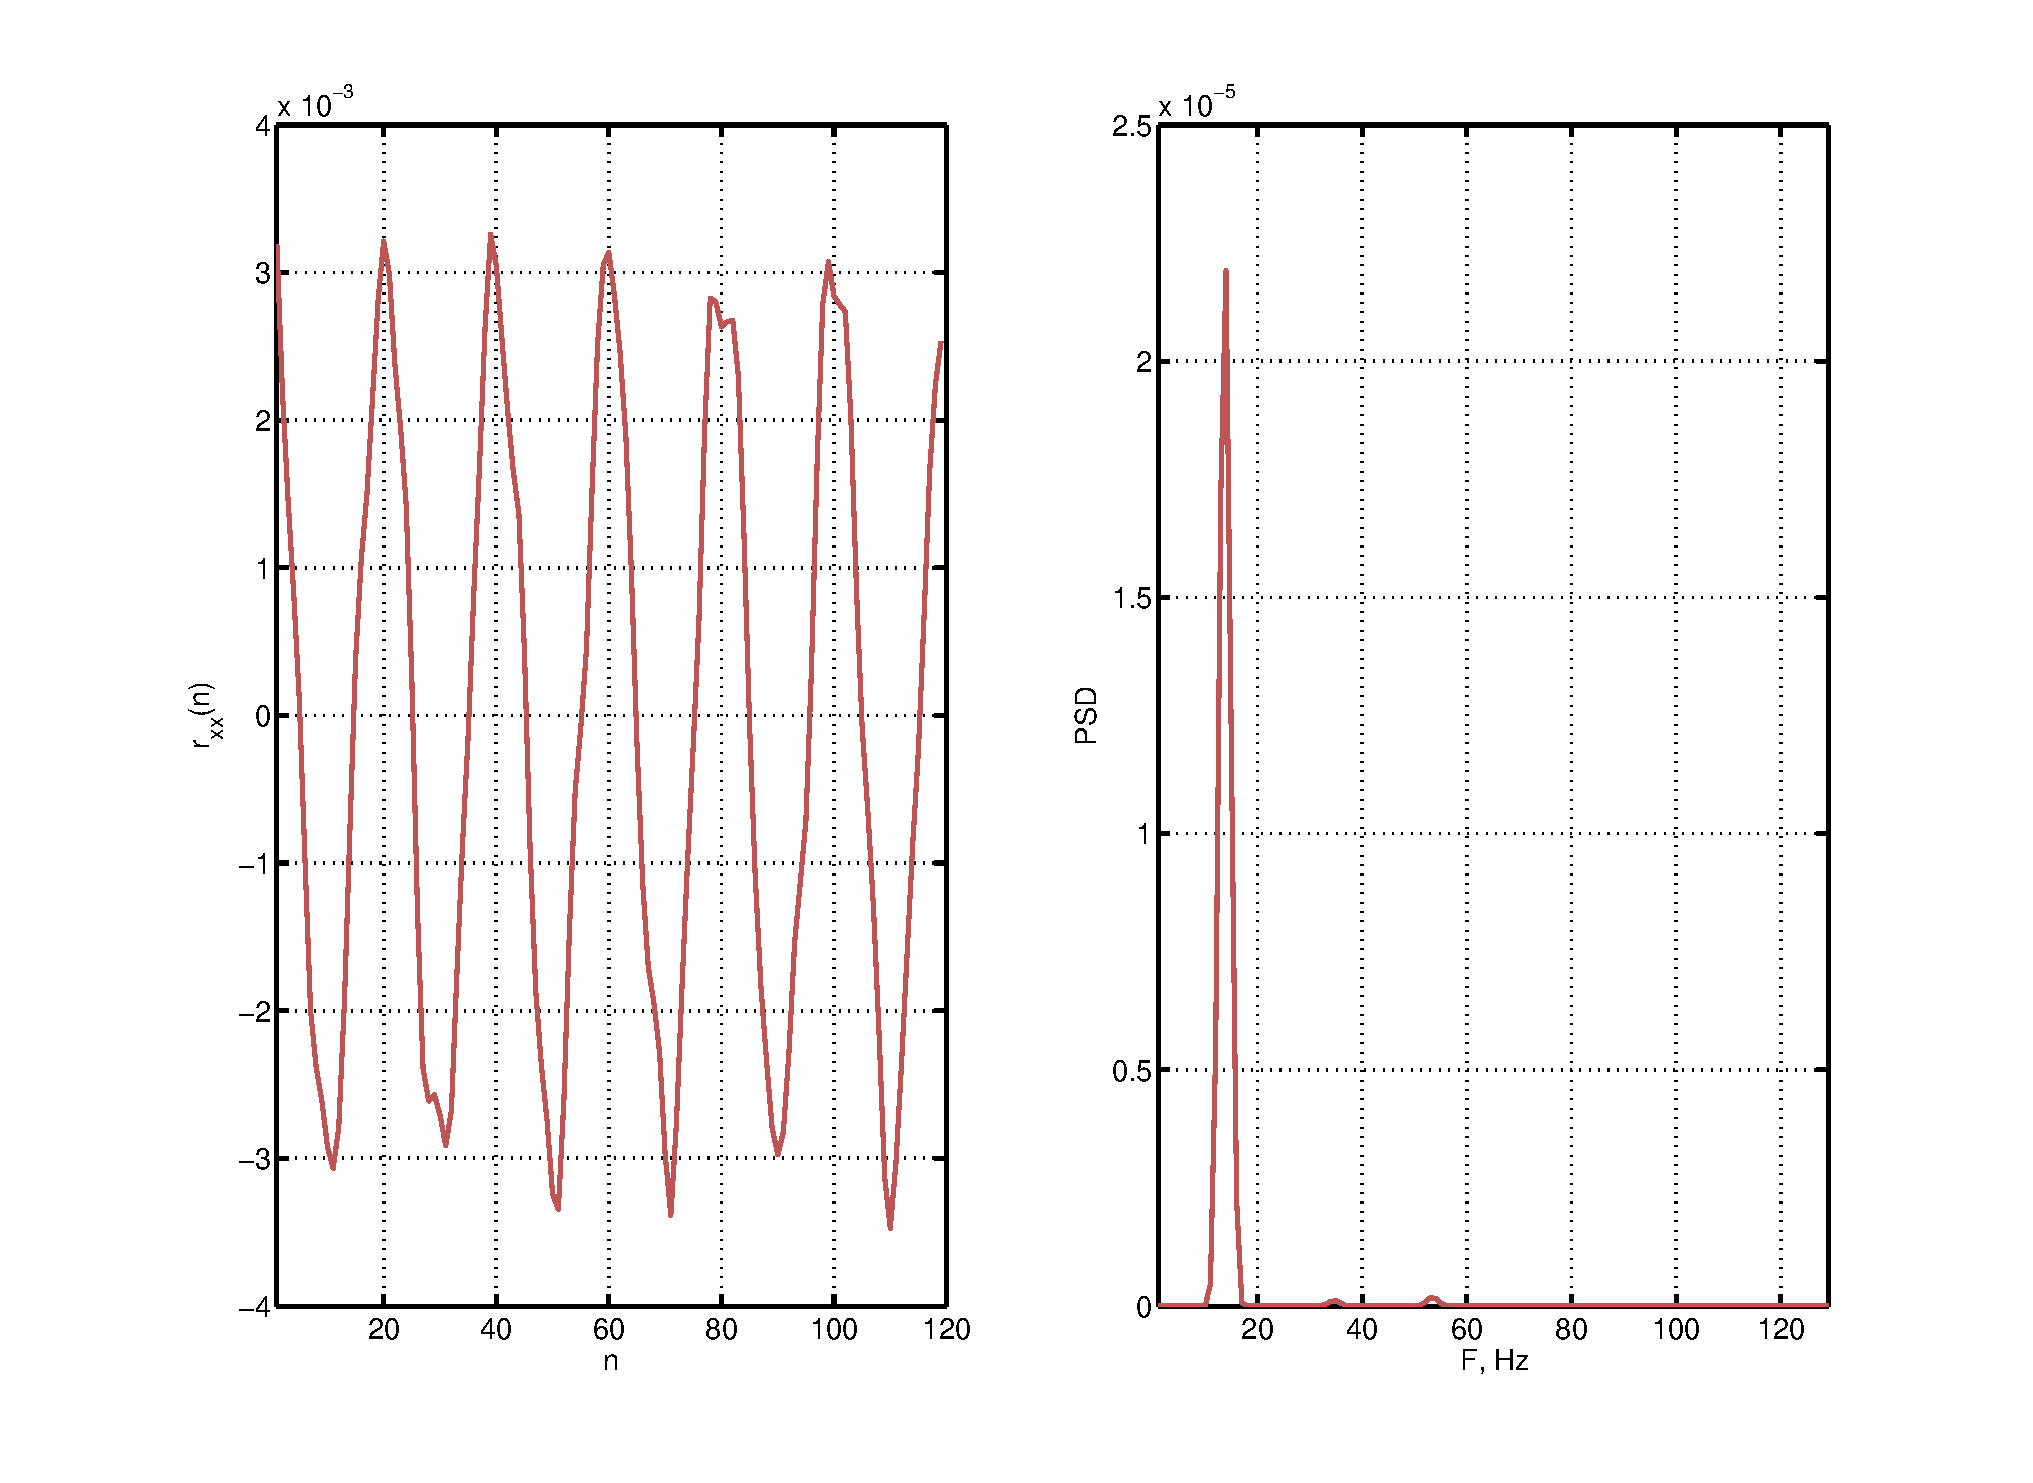
\includegraphics[width=1\linewidth]{acf_4_iter.eps}}
	\caption{Оценка АКФ на 4 итерации и ее спектр.}
	\label{pic:acf_4_iter}
\end{figure}

Представленный алгоритм позволяет значительно улучшить оценку АКФ. Следует отметить, что итеративный алгоритм вычисления АКФ так же
может быть использован для эффективного подавления окрашенного шума. В случае наличия интерференционной помехи в сигнале это дает
возможность получить несмещенную оценку частоты.

%%%%%%%%%%%%%%%%%
\section{Усовершенствованный итеративный алгоритм получения АКФ}
\label{sec_acf_fft}
Для приемников реального времени алгоритм, представленный в \cite{ostanin_akf} и приведенный в (\ref{sec_ostanin}), применять при оценке 
частоты ШПС не представляется возможным ввиду большого количества операций при вычислении АКФ.

Автором в \cite{my_acf} был предложен способ оптимизации алгоритма последовательного вычисления АКФ.
Для снижения вычислительных затрат указанный алгоритм предлагается реализовывать с использованием процедуры БПФ. 

Посчитаем АКФ для выражения (\ref{eq:acf_signal}).
\begin{equation}
	\label{eq:lpc_akf_n}
	\hat{r}_{xx}(n) = \sum \limits_{k=1}^{K} x(k)x(k+n) = \frac{A^2}{2} \cos{(\omega{n})} + \Delta_n \delta{(n)} + \mu{(n)}
\end{equation}

Здесь ${\Delta_n}$ - дисперсия шума ${n(k)}$, ${\mu{(n)}}$ - ошибка оценки АКФ, ${\delta{(n)}}$ - дельта-функция. Дисперсия ошибки
оценки ${\Delta_{\mu}}$ будет в ${K}$-раз меньше чем дисперсия ${\Delta_n}$ шума в принимаемом сигнале, где ${K}$ - интервал
осреднения оценки АКФ.

Используя оценку АКФ вместо исходной выборки, вновь получим оценку АКФ:
${r_{xx2}(n) = \frac{A^4}{8} \cos{(\omega n)} + \bar{N} \delta{(N)}}$,
где мощность шума оценки ${\bar{N}}$ - будет значительно меньше.

Амплитуда сигнала на итерации ${k}$ будет равна ${\frac{A^{2^k}}{2^{2^k-1}}}$. Увеличение отношения ОСШ по мощности можно
вычислить по уже приведенной формуле (\ref{eq:acf_snr_est}). 

Таким образом алгоритм можно представить в следующем виде.

Введем следующие обозначения: ${\bf{x}}$ – вектор входной смеси после повторной модуляции с ПСП, ${\bf{F}}$ – матрица прямого преобразования Фурье,
${\bf{F}^{-1}}$- матрица обратного преобразования Фурье.  Оценку АКФ на первом шаге можно получить следующим образом:
\begin{equation}
	\label{eq:akf_1}
	\hat{\bf{r}}_1 = \bf{F}^{-1}\left[ \bf{Fx} \cdot (\bf{Fx})^* \right] = \bf{F}^{-1} \left[ \left| \bf{Fx} \right| ^2 \right].
\end{equation}

Здесь знак ${(\cdot)}$  означает поэлементное перемножение векторов, ${\left| \bf{Fx} \right| ^2}$ - поэлементное возведение модуля комплексного числа в квадрат, ${*}$ -
комплексное сопряжение.  Следуя алгоритму, изложенному в \cite{ostanin_akf} вычислим оценку АКФ от ${\hat{\bf{r}}_1}$:
\begin{eqnarray}
	\label{eq:akf_2}
	\hat{\bf{r}}_2 & = & \bf{F}^{-1}\left[ \bf{F} \hat{\bf{r}}_1 \cdot (\bf{F} \hat{\bf{r}}_1)^* \right] = \nonumber \\
		& = & \bf{F}^{-1}	\left[ 
				\bf{FF}^{-1} \left[
						\left| \bf{Fx} \right| ^2
					\right]
						\cdot \left( \bf{FF}^{-1} \left[ \left| \bf{Fx} \right| ^2 \right]
					\right) ^*
			\right] = \nonumber \\
		& = & \bf{F}^{-1} \left[ \left| \bf{Fx} \right| ^2 \cdot \left[ \left| \bf{Fx} \right| ^2 \right] ^* \right] =  \nonumber \\
		& = & \bf{F}^{-1} \left[ \left| \bf{Fx} \right| ^4 \right].
\end{eqnarray}

Таким образом, уточненная оценка АКФ на ${K}$-ом шаге алгоритма, рассмотренного в \cite{ostanin_akf}
может быть получена без использования итераций с помощью выражения:
\begin{equation}
	\label{eq:akf_3}
	\hat{\bf{r}}_K = \bf{F}^{-1}\left[ \left| \bf{Fx} \right| ^{2^K} \right].
\end{equation}

Схематически алгоритм вычисления уточненной оценки АКФ на третьем шаге представлен на Рис. \ref{pic:akf_pic}.

\begin{figure}[h]
	\center\scalebox{0.7}{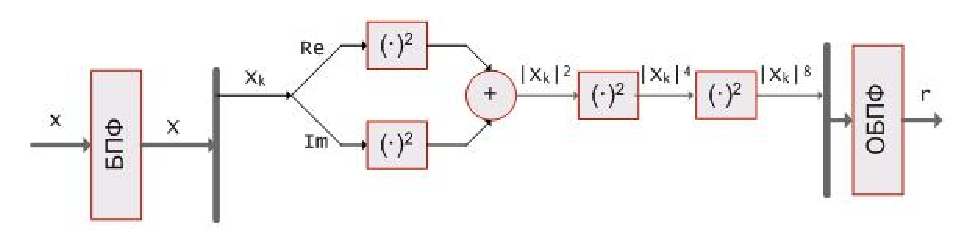
\includegraphics[width=1\linewidth]{akf_fft.eps}}
	\caption{Усовершенствованный итеративный алгоритм получения АКФ}
	\label{pic:akf_pic}
\end{figure}

Количество умножений действительных чисел, необходимых для оценки АКФ прямым методом без применения БПФ: 
\begin{equation}
	\label{eq:num_of_op_acf}
	OP_{ACF}=kN^2,
\end{equation}
где ${k}$  – количество итераций.

Количество умножений действительных чисел для получения оценки АКФ с применением усовершенствованного алгоритма вычисления оценки АКФ:
\begin{enumerate}
\item ${4NlogN}$ - действительных умножений - преобразование Фурье;
\item ${2N}$ - вычисление модуля комплексного числа;
\item ${N}$ - действительных умножений для каждой итерации (возведение в квадрат);
\item ${4NlogN}$ - действительных умножений – обратное преобразование Фурье. 
\end{enumerate}

Окончательно получаем:
\begin{equation}
	\label{eq:num_of_op_acf}
	OP_{ACF\_FFT}=8NlogN + (k+2)N.
\end{equation}

\section{Применение оконного взвешивания для оценки СПМ}

Так как в реальных условиях присутствует неопределенность по частоте, а длинна анализируемого объема данных конечна, пик на ПЧ в спектральной области не будет
представлять дельта функцию. Для улучшения свойств оценки СПМ представляется возможным использовать функции окон ${w(n)}$ - операция оконного взвешивания.
Свойства различных окон подробно рассмотрены, например, в \cite{shahtarin-spectrum-book, bolshakov-book}.

Наиболее популярными окнами являются: прямоугольное (равномерное), Бартлетта (треугольное), Ханна (косинус-квадрат), Хемминга (приподнятый косинус).

Оконная функция симметричного прямоугольного окна(\mbox{Рис. \ref{pic:win_rect}}) представляется выражением:
\begin{equation}
	\label{eq:rect_window}
	 w(n) = \begin{cases}
		1, |n| \le M; \\
		0, \mbox{в остальных случаях}.
		\end{cases}
\end{equation}
\begin{figure}[h]
	\center\scalebox{1}{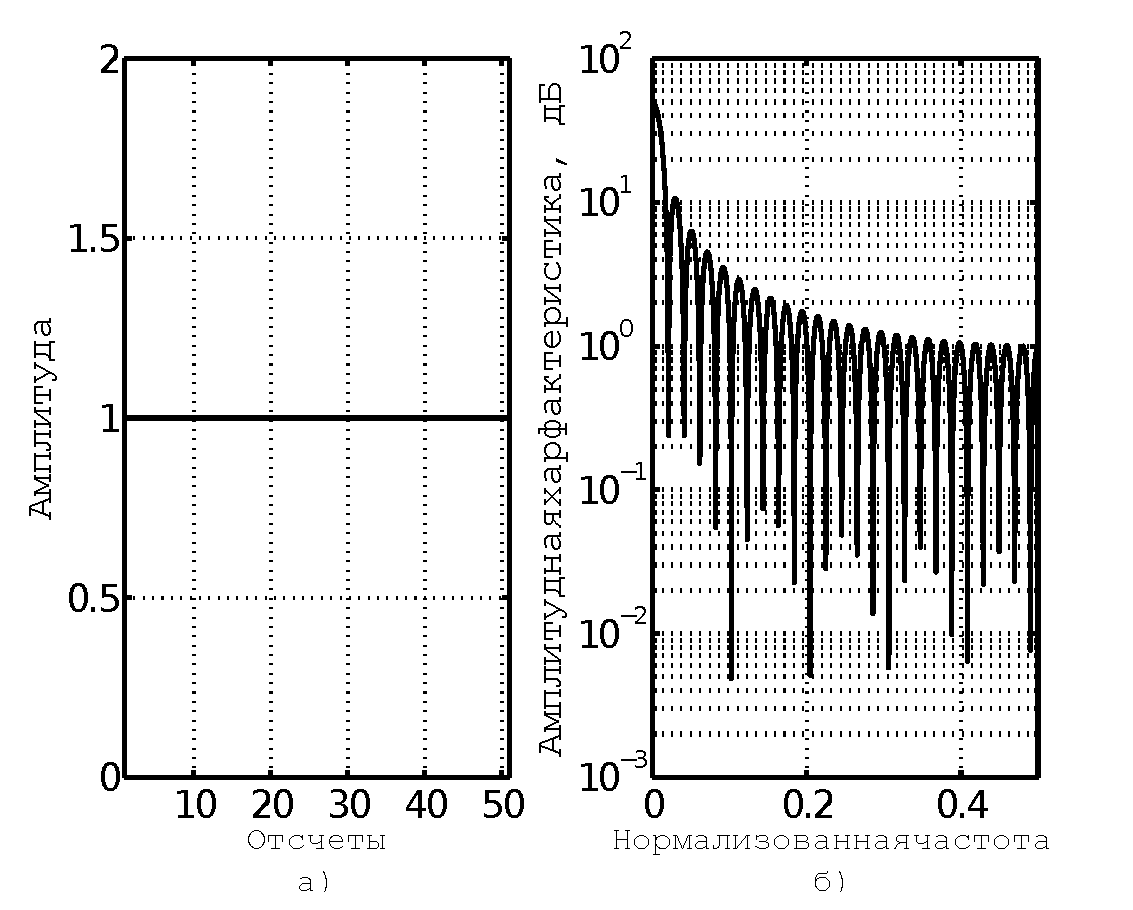
\includegraphics[width=1\linewidth]{various_windows_fig4.eps}}
	\caption{Прямоугольное окно. а - во временной области, б - в частотной}
	\label{pic:win_rect}
\end{figure}

Окно Бартлетта (\mbox{Рис. \ref{pic:win_bart}}) может быть представлено выражением:
\begin{equation}
	\label{eq:rect_bartlett}
	 w(n) = \begin{cases}
		1 - \frac{|n|}{M}, |n| \le M; \\
		0, \mbox{в остальных случаях}.
		\end{cases}
\end{equation}
\begin{figure}[h]
	\center\scalebox{1}{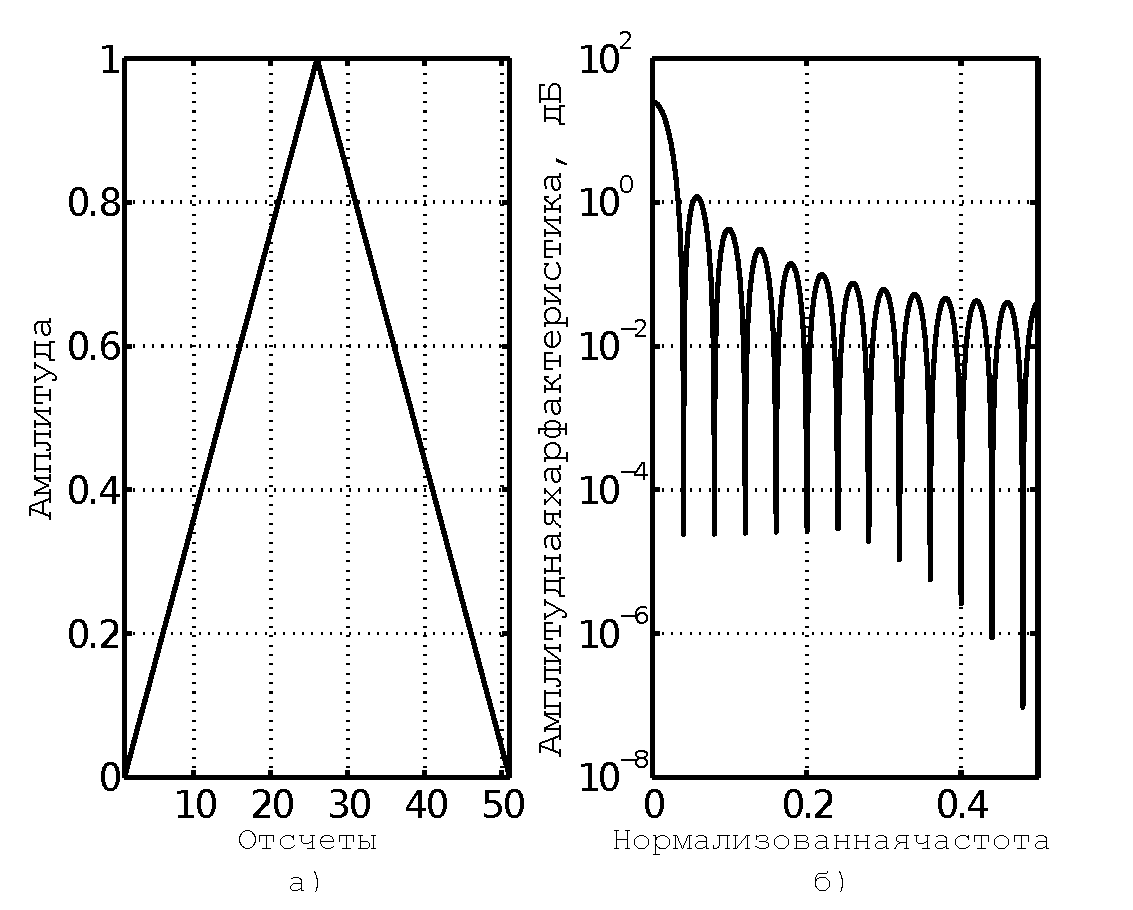
\includegraphics[width=1\linewidth]{various_windows_fig3.eps}}
	\caption{Окно Бартлетта. а - во временной области, б - в частотной}
	\label{pic:win_bart}
\end{figure}

Окно Хемминга (\mbox{Рис. \ref{pic:win_hamming}}) может быть представлено выражением:
\begin{equation}
	\label{eq:rect_hamming}
	 w(n) = \begin{cases}
		0.54 - 0.46\cos \left( 2 \pi \frac{n}{M} \right), 0 \le n \le M; \\
		0, \mbox{в остальных случаях}.
		\end{cases}
\end{equation}
\begin{figure}[h]
	\center\scalebox{1}{\includegraphics[width=1\linewidth]{various_windows_fig2.eps}}
	\caption{Окно Хемминга. а - во временной области, б - в частотной}
	\label{pic:win_hamming}
\end{figure}

Окно Ханна (\mbox{Рис. \ref{pic:win_hann}}) может быть представлено выражением:
\begin{equation}
	\label{eq:rect_hann}
	 w(n) = \begin{cases}
		0.5 \left( 1 - \cos\left( 2 \pi \frac{n}{M} \right) \right) \\
		0, \mbox{в остальных случаях}.
		\end{cases}
\end{equation}
\begin{figure}[h]
	\center\scalebox{1}{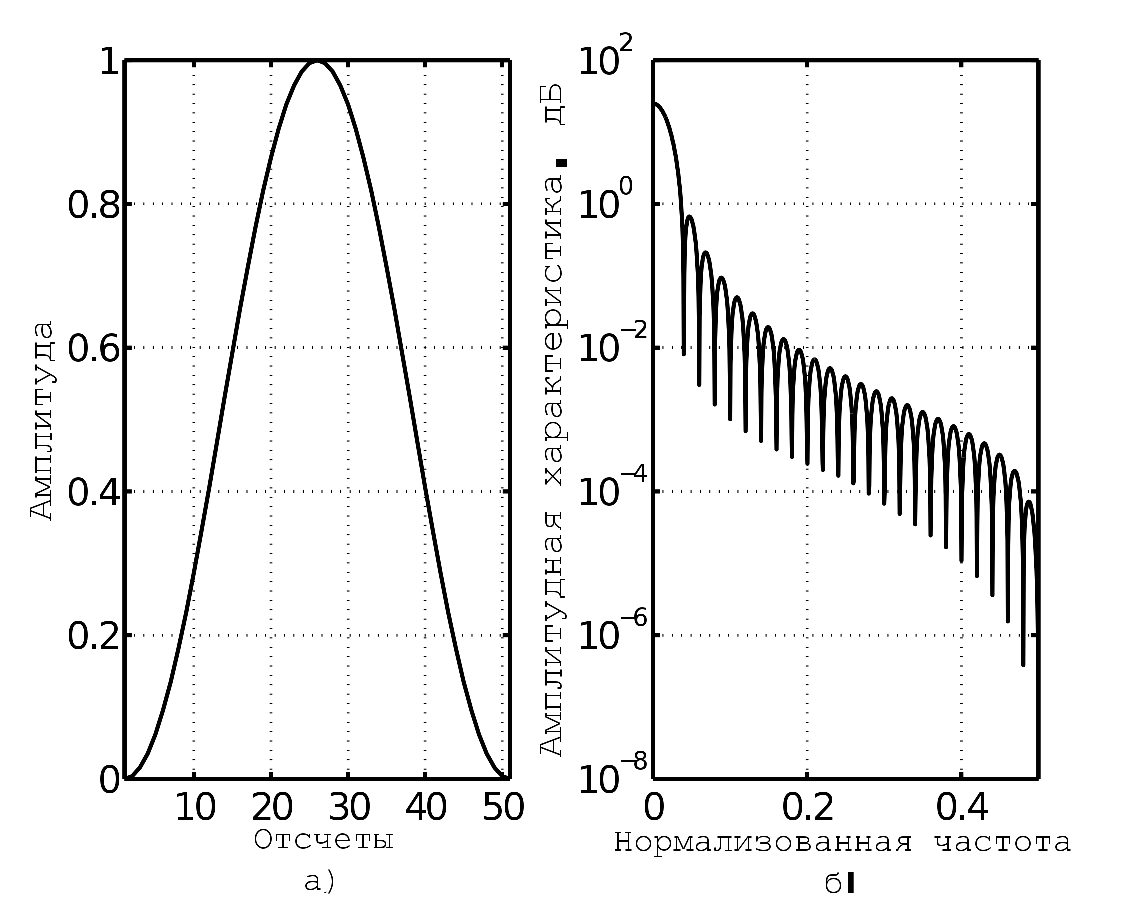
\includegraphics[width=1\linewidth]{various_windows_fig1.eps}}
	\caption{Окно Ханна. а - во временной области, б - в частотной}
	\label{pic:win_hann}
\end{figure}

Основными недостатками прямоугольного окна являются: наличие ложных максимумов, знакопеременность. В тоже время прямоугольное окно имеет самую малую ширину главного лепестка, но
одновременно с этим достаточно большие и медленно убывающие знакопеременные боковые лепестки. Окна Бартлетта и Ханна всюду положительны, а окно Хемминга положительно не всюду, однако
первый боковой лепесток составляет 0.021 высоты основного лепестка. Этим обусловлена популярность данного окна в задачах спектрального анализа.

В виду того, что задача итеративной оценки АКФ не является стандартной задачей спектрального анализа необходимо провести дополнительные исследования. В процессе
диссертационной работы было проведено численное моделирование применения разных окон в алгоритме итеративного вычисления оценки АКФ.

{\bf{\textit{Применение оконного взвешивания в задаче итеративного вычисления АКФ}}}

Из \cite{bolshakov-book} известно, что прямоугольное окно является самым узким, но вместе с тем имеет достаточно существенные боковые лепестки. В задаче итеративной оценки
АКФ, функция умножается несколько раз поточечно в частотном домене. Это позволяет предположить, что боковые лепестки будут увеличивать свое значение медленнее основного.
Для проверки данной гипотезы был проведен вычислительный эксперимент.

%%%%%%
\section{Практические аспекты применения}
\label{lab:sec2_windows}

При практической реализации алгоритма оценки частоты на основе АР-модели важным является качество оценки АКФ функции. В предложенном алгоритме итеративной оценки АКФ,
в случае блочной обработки данных, будет наблюдаться эффект растекания спектра вследствии того, что ПЧ не является кратной частоте дискретизации. В процессе диссертационного
исследования было проведено численное моделирование применения различных комбинаций оконных функций и различных длин блоков нулей, при вычислении БПФ для повышения
разрешающей способности, как это рекомендовано для алгоритмов оценки СПМ \cite{bolshakov-book}.

В \cite{bolshakov-book} отмечено, что для повышения разрешения в методах, основанных на корреляционных функциях, можно дополнять исходную последовательность нулями.
Но, с другой стороны, при добавлении нулей ко входной последовательности количество операций для оценки АКФ возрастает. Таким образом необходимо провести дополнительное
исследование для оценки минимально возможного количества нулей, которые необходимо добавить ко входной последовательности для повышения точности оценки частоты,
удовлетворяющей входной расстройке ФАПЧ.

Для оценки количества нулей, необходимых для попадания оценки частоты в диапазон допустимой входной расстройки ФАПЧ был проведен вычислительный эксперимент. В качестве диапазона
ОСШ был взят диапазон от -30 дБ до 5 дБ, количество нулей в диапазоне ${[0, 6N]}$, где ${N}$ - длинна данных. Допустимая входная расстройка была взята в диапазоне ${[-40, 40]}$ Гц.
Опыт проводился на фоне АБГШ без МКИ. Оценивалось СКО оценки при использовании разных типов окон и разного количества итераций пересчета АКФ.

На Рис. \ref{pic:fft2_1} представлено моделирование для последовательности дополненной нулями до длинны ${2N}$ с применением различных оконных функций:
прямоугольного окна, окна Хемминга, окна Блекмана и окна Ханна при одной итерации уточнения АКФ.
\begin{figure}[h]
	\center\scalebox{0.7}{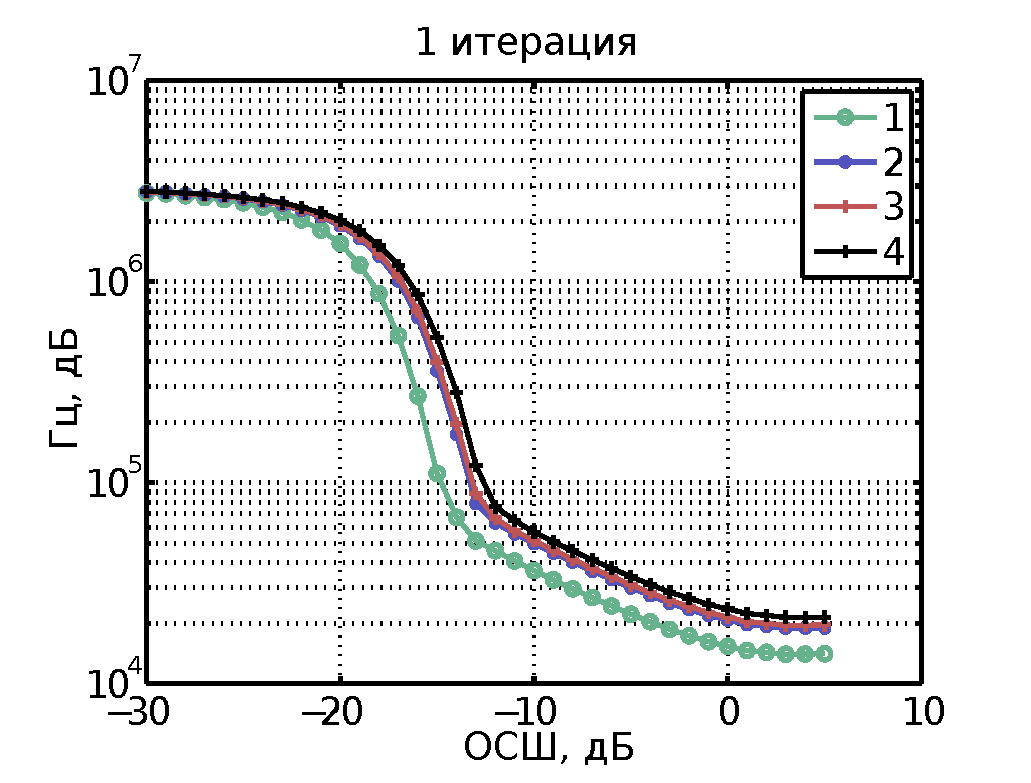
\includegraphics[width=1\linewidth]{fft2_1.eps}}
	\caption{\\СКО оценки частоты. 1 - прямоугольное окно,\\2 - окно Хемминга, 3 - окно Блекмана, 4 - окно Ханна.}
	\label{pic:fft2_1}
\end{figure}

На Рис. \ref{pic:fft2_2} представлено моделирование для последовательности дополненной нулями до длинны ${2N}$ с применением различных оконных функций:
прямоугольного окна, окна Хемминга, окна Блекмана и окна Ханна при двух итерациях уточнения АКФ.
\begin{figure}[h]
	\center\scalebox{0.7}{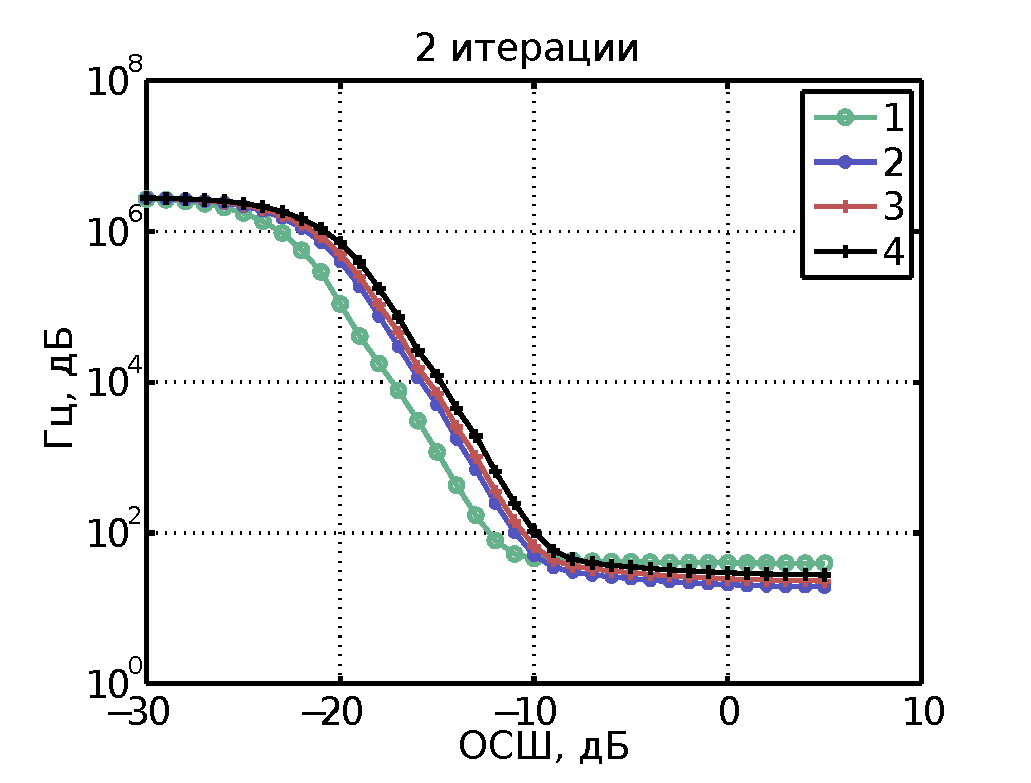
\includegraphics[width=1\linewidth]{fft2_2.eps}}
	\caption{\\СКО оценки частоты. 1 - прямоугольное окно,\\2 - окно Хемминга, 3 - окно Блекмана, 4 - окно Ханна.}
	\label{pic:fft2_2}
\end{figure}

На Рис. \ref{pic:fft2_3} представлено моделирование для последовательности дополненной нулями до длинны ${2N}$ с применением различных оконных функций:
прямоугольного окна, окна Хемминга, окна Блекмана и окна Ханна при трех итерациях уточнения АКФ.
\begin{figure}[h]
	\center\scalebox{0.7}{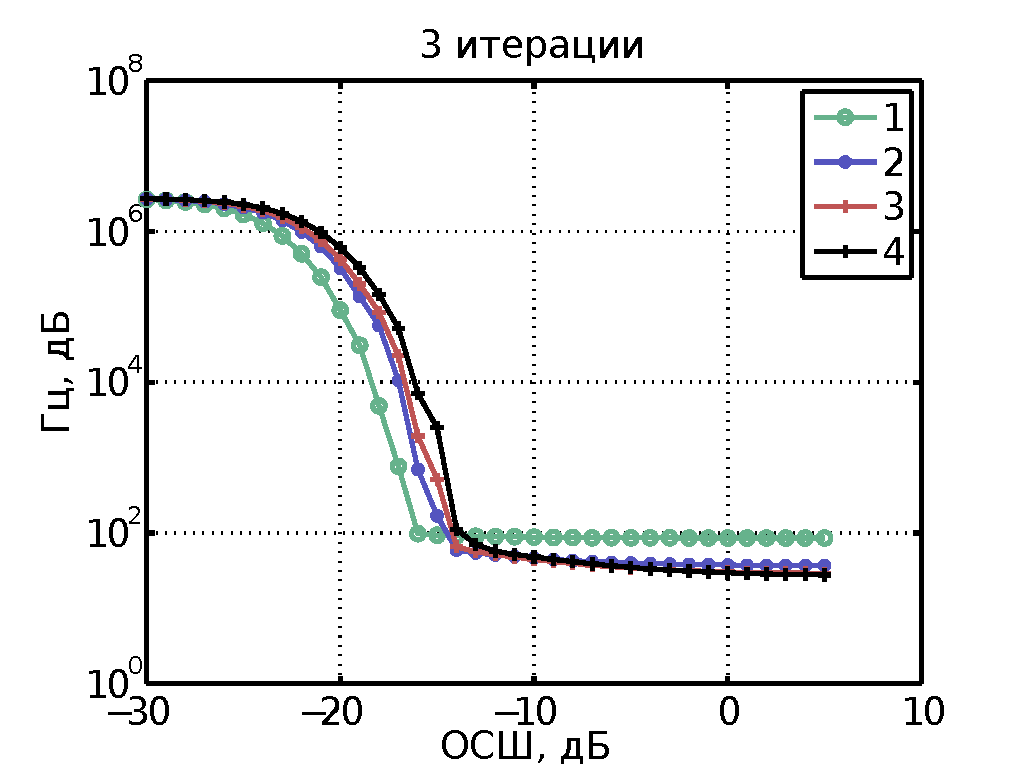
\includegraphics[width=1\linewidth]{fft2_3.eps}}
	\caption{\\СКО оценки частоты. 1 - прямоугольное окно,\\2 - окно Хемминга, 3 - окно Блекмана, 4 - окно Ханна.}
	\label{pic:fft2_3}
\end{figure}

Из Рис. \ref{pic:fft2_1}, \ref{pic:fft2_2}, \ref{pic:fft2_3} видно, что лучшие результаты показывает подход с применением прямоугольного окна. На Рис. \ref{pic:fft2_rect_1_2_3}
представлен график СКО оценки частоты для одной, двух и трех итераций уточнения АКФ с применением прямоугольного окна. Из \mbox{Рис. \ref{pic:fft2_1}-\ref{pic:fft2_3}}  видно, что большее
количество итераций уточнения позволяет более точно получать оценку на низких ОСШ, вместе с тем точность оценки несколько снижается для ОСШ выше \mbox{-10 дБ.}
\begin{figure}[h]
	\center\scalebox{0.7}{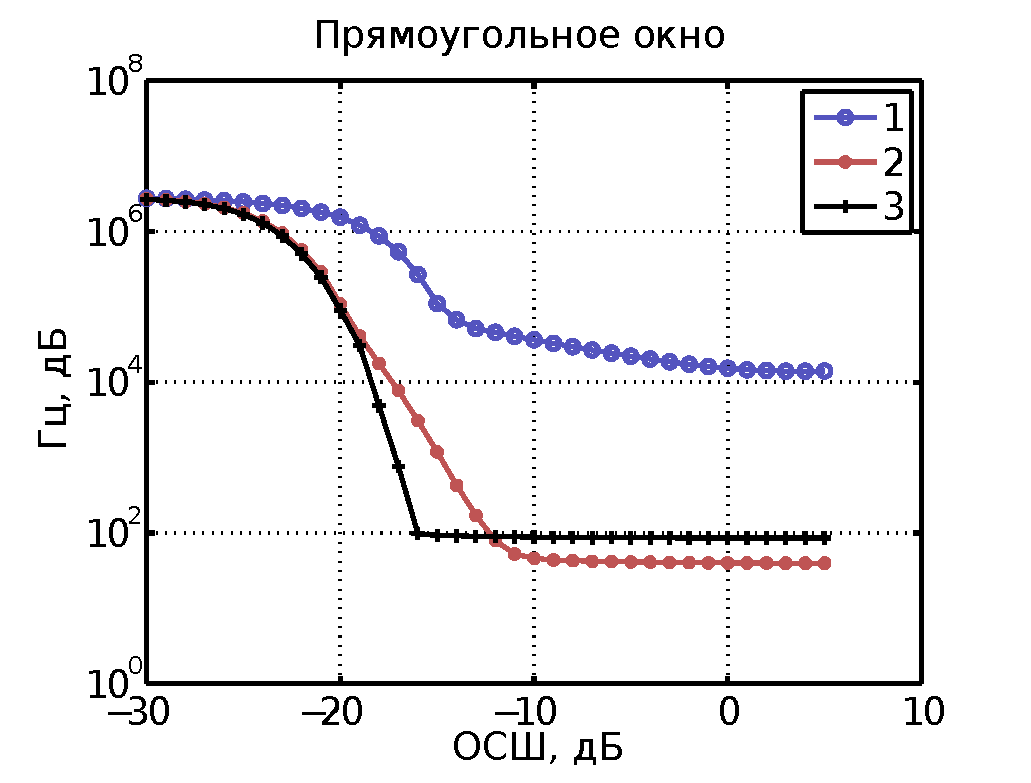
\includegraphics[width=1\linewidth]{fft2_rect_1_2_3.eps}}
	\caption{\\СКО оценки частоты. 1 - одна итерация пересчета АКФ,\\2 - две итерации пересчета АКФ, 3 - три итерации пересчета АКФ.}
	\label{pic:fft2_rect_1_2_3}
\end{figure}

Представляется интересным изучить влияние длинны блока нулей, дополняющий входную смесь, на СКО оценки частоты. Для решения данной задачи было проведено еще одно моделирование.
На Рис. \ref{pic:fft4_1} представлено моделирование для последовательности дополненной нулями до длинны ${4N}$ с применением различных оконных функций:
прямоугольного окна, окна Хемминга, окна Блекмана и окна Ханна при одной итерации уточнения АКФ.
\begin{figure}[h]
	\center\scalebox{0.7}{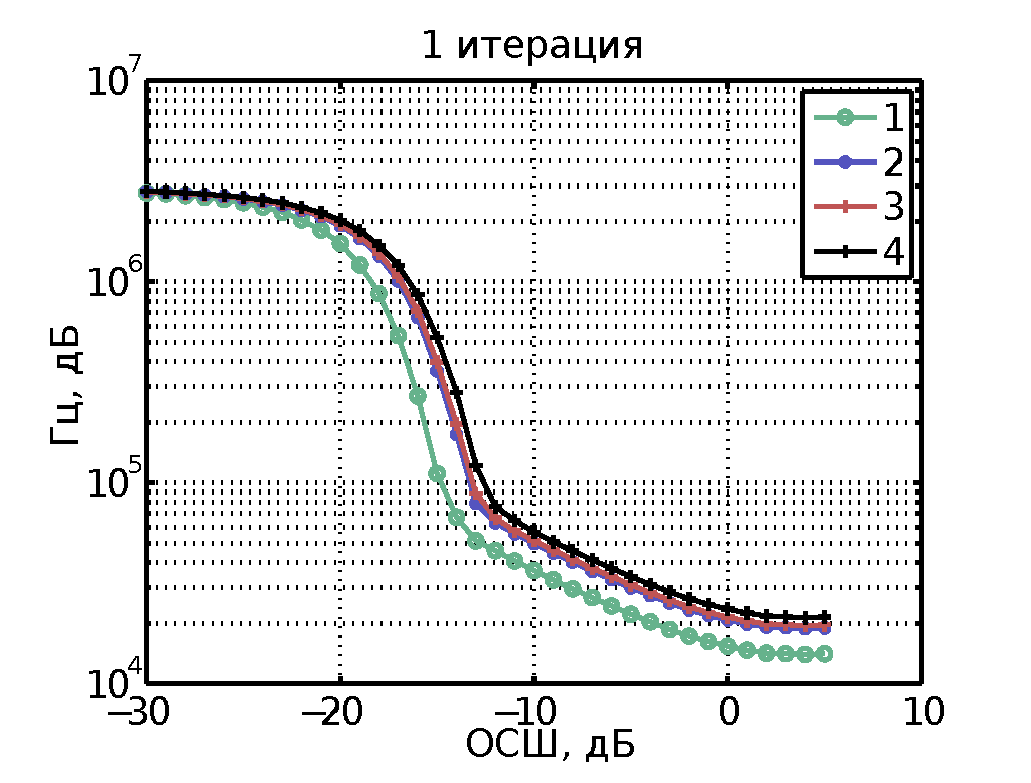
\includegraphics[width=1\linewidth]{fft4_1.eps}}
	\caption{\\СКО оценки частоты. 1 - прямоугольное окно,\\2 - окно Хемминга, 3 - окно Блекмана, 4 - окно Ханна.}
	\label{pic:fft4_1}
\end{figure}

На Рис. \ref{pic:fft4_2} представлено моделирование для последовательности дополненной нулями до длинны ${4N}$ с применением различных оконных функций:
прямоугольного окна, окна Хемминга, окна Блекмана и окна Ханна при двух итерациях уточнения АКФ.
\begin{figure}[h]
	\center\scalebox{0.7}{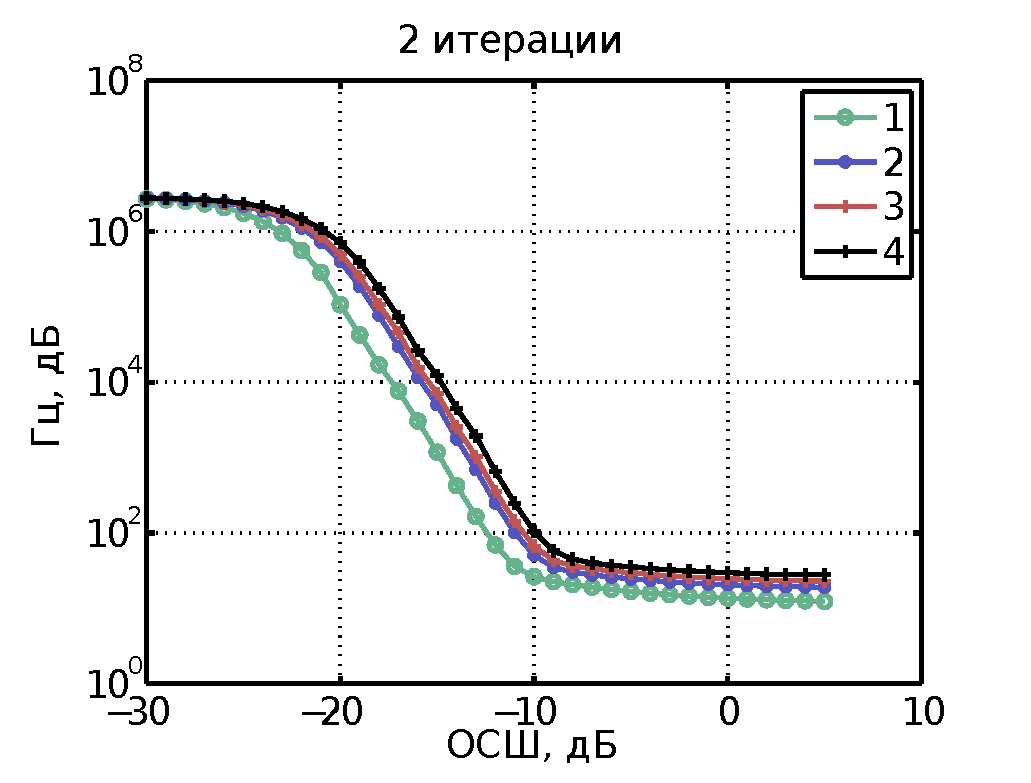
\includegraphics[width=1\linewidth]{fft4_2.eps}}
	\caption{\\СКО оценки частоты. 1 - прямоугольное окно,\\2 - окно Хемминга, 3 - окно Блекмана, 4 - окно Ханна.}
	\label{pic:fft4_2}
\end{figure}

На Рис. \ref{pic:fft4_3} представлено моделирование для последовательности дополненной нулями до длинны ${4N}$ с применением различных оконных функций:
прямоугольного окна, окна Хемминга, окна Блекмана и окна Ханна при трех итерациях уточнения АКФ.
\begin{figure}[h]
	\center\scalebox{0.7}{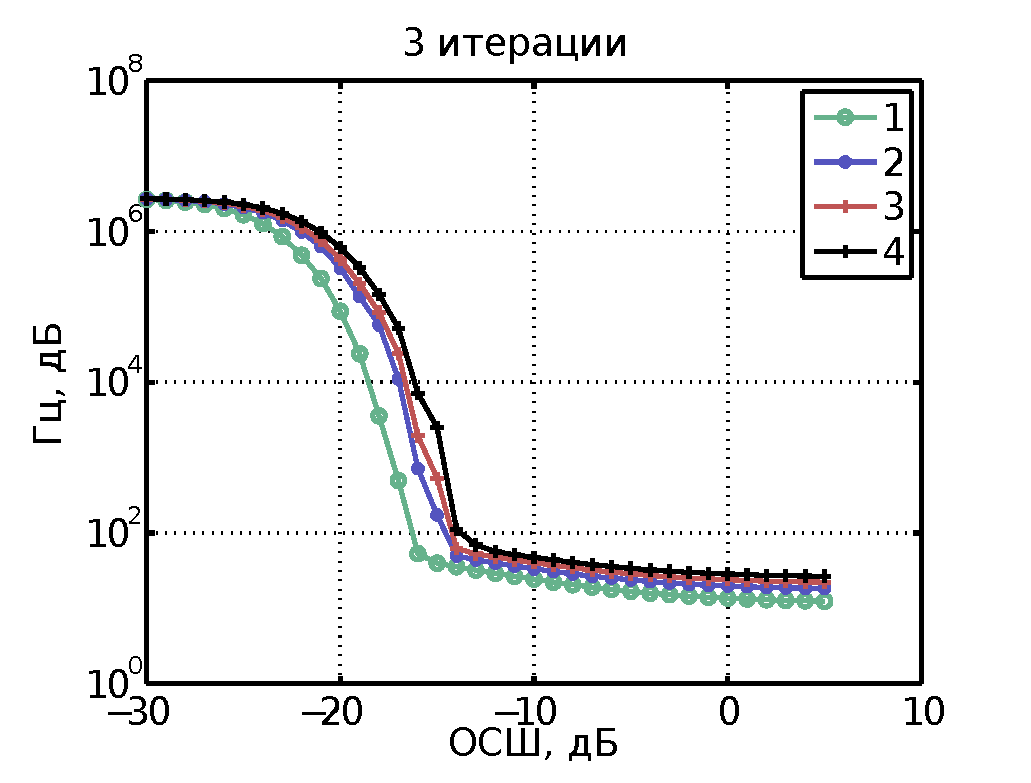
\includegraphics[width=1\linewidth]{fft4_3.eps}}
	\caption{\\СКО оценки частоты. 1 - прямоугольное окно,\\2 - окно Хемминга, 3 - окно Блекмана, 4 - окно Ханна.}
	\label{pic:fft4_3}
\end{figure}

Из Рис. \ref{pic:fft4_1}, \ref{pic:fft4_2}, \ref{pic:fft4_3} видно, что, также, как и в случае с длинной ${2N}$, лучшие результаты показывает подход с применением прямоугольного окна.
На Рис. \ref{pic:fft4_rect_1_2_3}
представлен график СКО оценки частоты для одной, двух и трех итераций уточнения АКФ с применением прямоугольного окна для блока данных, дополненного нулями до длинны ${4N}$.
Из графиков видно, что большее количество итераций уточнения позволяет более точно получать оценку на низких ОСШ, но в случае с длинной данных ${2N}$ оценки снижалась при
возрастании ОСШ при длине ${4N}$ данного эффекта не наблюдается.
\begin{figure}[h]
	\center\scalebox{0.7}{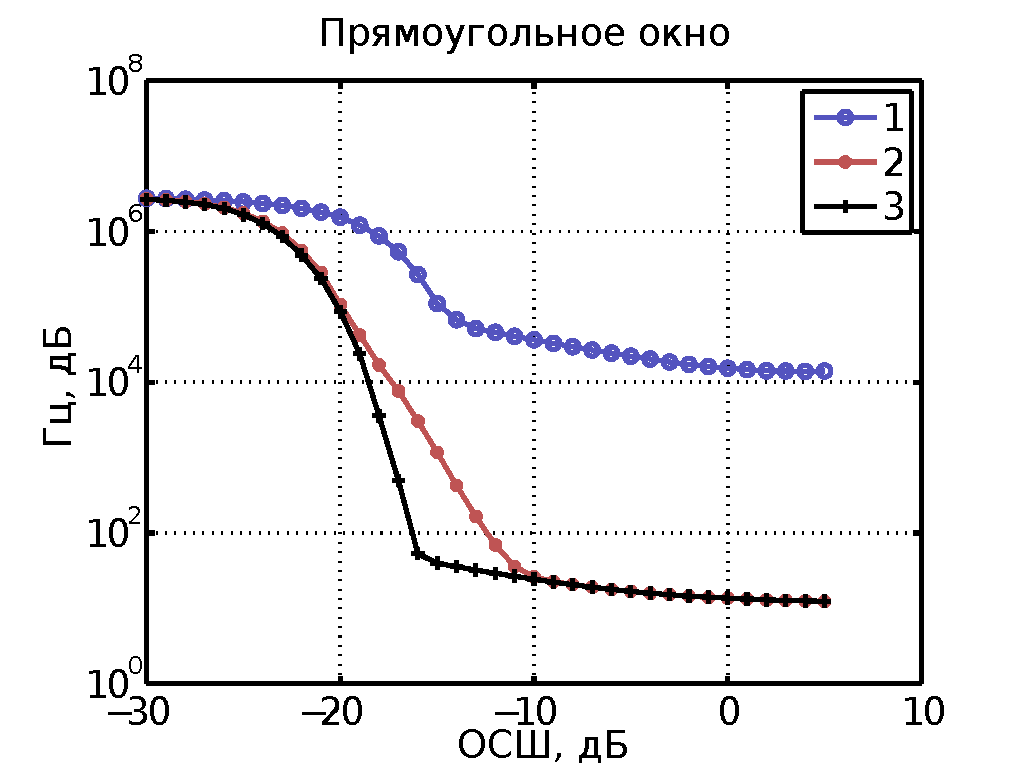
\includegraphics[width=1\linewidth]{fft4_rect_1_2_3.eps}}
	\caption{\\СКО оценки частоты. 1 - одна итерация пересчета АКФ,\\2 - две итерации пересчета АКФ, 3 - три итерации пересчета АКФ.}
	\label{pic:fft4_rect_1_2_3}
\end{figure}

Из приведенных результатов можно заключить, что наилучшими характеристиками для сигналов с ОСШ ${\le}$ -15 дБ обладает прямоугольное окно. Для сигналов с ОСШ ${\ge}$ 
-15 дБ целесообразно использовать оконное взвешивание. Стоит отметить, что худшими результатами для низких ОСШ (менее 15 дБ) обладает окно Ханна.
Так же из приведенных результатов можно сделать вывод что использование БПФ длиной ${2N}$ нецелесообразно в виду низкой
точности, длины ${4N}$ и ${8N}$ обладают практически одинаковыми характеристиками. Таким образом целесообразно использовать длину ${4N}$. Наилучшие результаты были получены при
использовании трех итераций уточнения АКФ. На Рис. \ref{pic:2vs4vs8} представлена сводка результатов для прямоугольного окна, трех итераций уточнения АКФ и различных длин БПФ.

\begin{figure}[h]
	\center\scalebox{0.7}{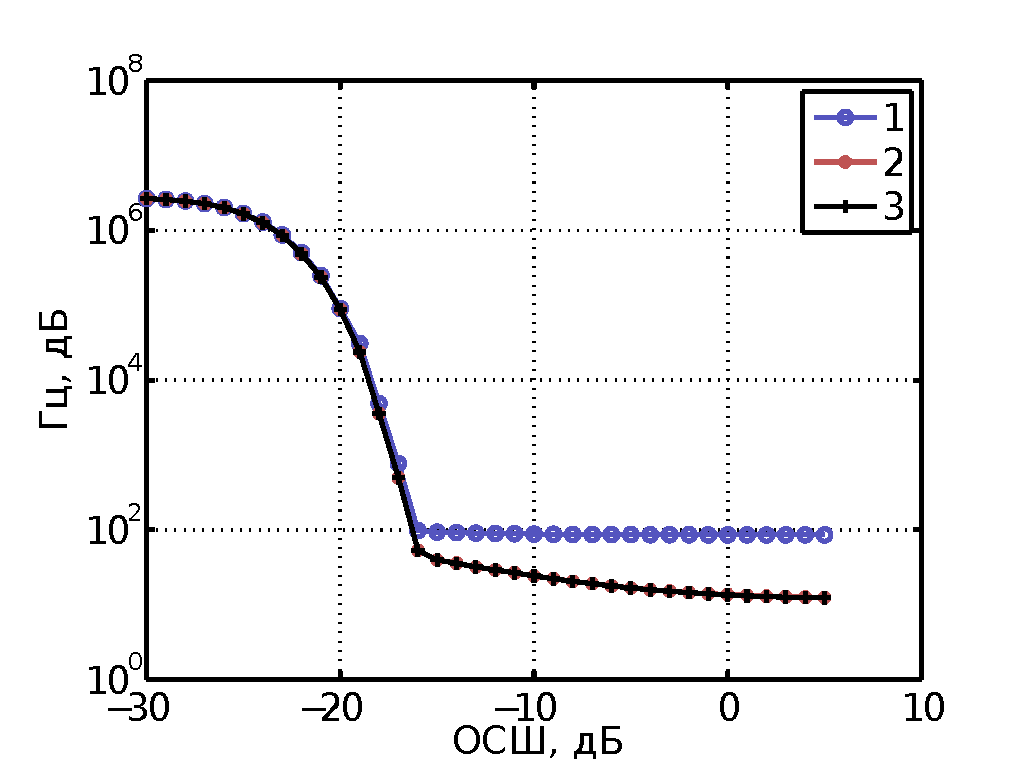
\includegraphics[width=1\linewidth]{2vs4vs8.eps}}
	\caption{\\СКО оценки частоты. 1 - БПФ длиной ${2N}$,\\2 - БПФ длиной ${4N}$, 3 - БПФ длиной ${8N}$.}
	\label{pic:2vs4vs8}
\end{figure}

%На Рис. \ref{pic:acf_3d} представлен трехмерный график обобщающий опыты проведенные ранее для прямоугольного окна. Из графика видно что длинна БПФ равная ${2N}$ позволяет получить оценку
%с одинаковой точностью для диапазона ${[0, 20]}$ дБ.
%\begin{figure}[h]
%	\center\scalebox{0.8}{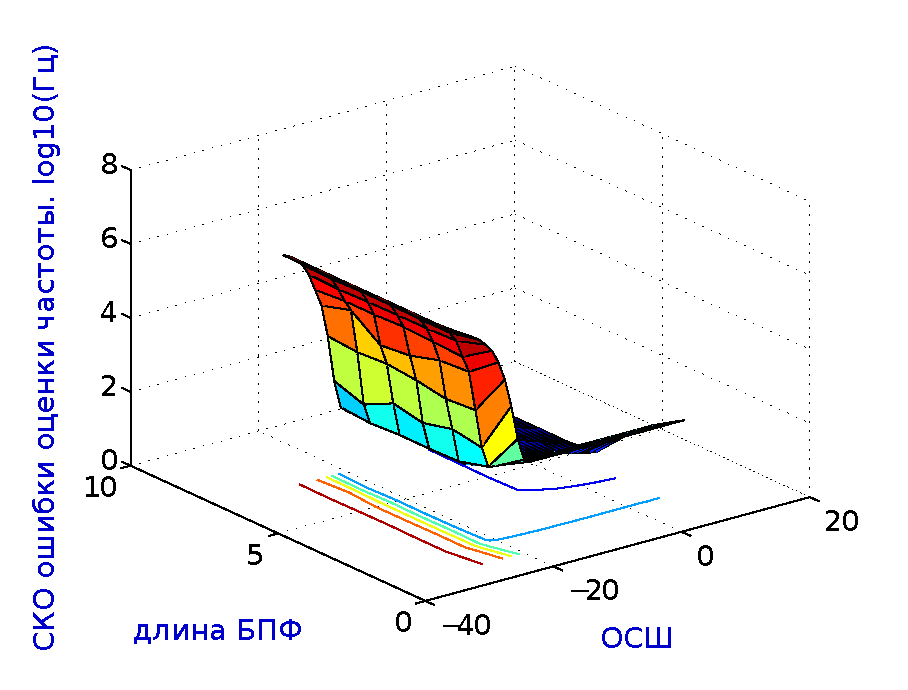
\includegraphics[width=1\linewidth]{acf_3d.eps}}
%	\caption{СКО оценки частоты.}
%	\label{pic:acf_3d}
%\end{figure}

\section{Выводы по Главе 2}

\begin{itemize}
\item АКФ от гармонического сигнала является гармоническим сигналом той же частоты, но с более высоким ОСШ, что позволяет использовать АКФ, полученную итеративно,
	для оценки частоты гармонических компонент, присутствующих во входной смеси.

\item Задача итеративного вычисления оценки АКФ может быть эффективно решена в базисе Фурье.

\item Задача повышения точности оценки частоты в методах с применением АКФ может быть решена при помощи дополнения входной последовательности нулями.

\item В результате имитационного моделирования было получено значение количества нулей и тип функции оконного взвешивания, а также количество итераций уточнения АКФ,
	позволяющих получить оценку частоты, удовлетворяющую входной расстройке ФАПЧ, с использованием АР-модели, при минимальных вычислительных затратах для низких ОСШ.
	Использование прямоугольного окна при дополнении блоком в ${3N}$ нулей (общая длинна последовательности ${4N}$) и трех итерациях уточнения АКФ дает лучше результаты
	для  \mbox{ОСШ ${\le}$ -15 дБ.}

\item Результаты имитационного моделирования показали, что использование окна Ханна для низких ОСШ (менее -15 дБ) дает худшие результаты в сравнении с прямоугольным
	окном и окнами Блекмена и Хемминга.

\end{itemize}

%%%%%%
\clearpage
\addtocontents{toc}{\hfill\par}			% добавить Стр. над номерами страниц
\addtocontents{toc}{~\hfill{Стр.}\par}			% добавить Стр. над номерами страниц
%%%%%%

\clearpage
